%%%%%%%%%%%%%%%%%%%%%%%%%%%%%%%%%%%%%%%%%%%%%%%%%%%%%%%%%%%%%%%%%%%%%%%%%%%%%%%
%
%  An AI Course Scheduler: Hybrid Constraint Satisfaction and
%  Probabilistic Preference Modeling for Personalized Academic Planning
%
%  CS 4710 - Artificial Intelligence, Final Report (Team 1)
%  Formatted in the style of an ICML submission.
%
%%%%%%%%%%%%%%%%%%%%%%%%%%%%%%%%%%%%%%%%%%%%%%%%%%%%%%%%%%%%%%%%%%%%%%%%%%%%%%%

\documentclass[10pt,letterpaper]{article}

% ----- Packages ---------------------------------------------------------------
\usepackage[letterpaper,margin=1in]{geometry}
\usepackage{times}
\usepackage{microtype}
\usepackage[T1]{fontenc}
\usepackage[utf8]{inputenc}
\usepackage{amsmath,amssymb,amsfonts}
\usepackage{graphicx}
\usepackage{booktabs}
\usepackage{multirow}
\usepackage{multicol}
\usepackage{hyperref}
\usepackage{url}
\usepackage{xcolor}
\usepackage{enumitem}
\usepackage{tikz}
\usetikzlibrary{arrows.meta,positioning,shapes.geometric,fit,backgrounds}
\usepackage{caption}
\usepackage{titlesec}
\usepackage{authblk}
\usepackage{algorithm}
\usepackage{algpseudocode}

% ----- ICML-style header ------------------------------------------------------
\usepackage{fancyhdr}
\pagestyle{fancy}
\fancyhf{}
\fancyhead[L]{\small\itshape An AI Course Scheduler}
\fancyhead[R]{\small\itshape CS 4710 Final Report, Spring 2026}
\renewcommand{\headrulewidth}{0.4pt}
\fancyfoot[C]{\thepage}

% ----- Hyperref styling -------------------------------------------------------
\hypersetup{
  colorlinks=true,
  linkcolor=black,
  citecolor=blue!60!black,
  urlcolor=blue!60!black,
}

% ----- Section formatting (ICML-like) -----------------------------------------
\titleformat{\section}{\normalfont\large\bfseries}{\thesection}{0.7em}{}
\titleformat{\subsection}{\normalfont\normalsize\bfseries}{\thesubsection}{0.7em}{}
\titlespacing*{\section}{0pt}{1.4ex plus .4ex minus .2ex}{0.6ex plus .2ex}
\titlespacing*{\subsection}{0pt}{1.0ex plus .3ex minus .2ex}{0.4ex plus .2ex}

% ----- Title and author block (ICML-like) -------------------------------------
\renewcommand{\Authsep}{\quad}
\renewcommand{\Authand}{\quad}
\renewcommand{\Authands}{\quad}
\setlength{\affilsep}{0.6em}

% ----- Convenience macros -----------------------------------------------------
\newcommand{\code}[1]{\texttt{\small #1}}
\newcommand{\eg}{\emph{e.g.,}}
\newcommand{\ie}{\emph{i.e.,}}

% ==============================================================================
\begin{document}

\twocolumn[
  \begin{@twocolumnfalse}
    \begin{center}
      {\LARGE\bfseries An AI Course Scheduler: Hybrid Constraint\\[2pt]
       Satisfaction and Probabilistic Preference Modeling\\[2pt]
       for Personalized Academic Planning\par}
      \vspace{0.6em}
      {\large\itshape CS 4710 -- Artificial Intelligence \\ Final Project Report, Team~1\par}
      \vspace{0.8em}
      {\normalsize
        Liam Baird \quad
        Hugo Barnes \quad
        Alex Chen \quad
        Matthew Heilman \\[2pt]
        \small University of Virginia, School of Engineering and Applied Science\\
        \small \texttt{\{lab9rfn, hsb4rh, axc6rfn, mwh4kc\}@virginia.edu}\par}
      \vspace{0.6em}
    \end{center}

    \begin{abstract}
      \noindent
      Course registration is a recurring source of friction for undergraduates:
      students must reconcile graduation requirements, prerequisite chains,
      time-slot conflicts, and personal preferences over difficulty,
      instructor, and topic, often through hours of manual trial and error.
      We present an \textbf{AI Course Scheduler} that produces complete,
      conflict-free course schedules tailored to an individual student.
      The system combines a regex-based prerequisite parser and topological
      sort, an LLM-driven sentiment analyzer over course reviews, a
      backtracking constraint solver, a Bayesian network for preference
      modeling, and a neural network that scores candidate schedules.
      Outputs are accompanied by natural-language justifications generated
      by a locally-hosted Qwen~2.5 7B model (via Ollama) running on the UVA
      Rivanna HPC cluster. We synthesize a corpus of \textbf{312 course
      sections} and \textbf{1{,}620 reviews} grounded in publicly available
      \emph{TheCourseForum} content, and show that targeted bias correction
      and structured prompt templating substantially improve recommendation
      quality. Our final pipeline produces a 15-credit, conflict-free
      schedule with an overall preference score of 68\,\% on representative
      student profiles.
    \end{abstract}
    \vspace{1.0em}
  \end{@twocolumnfalse}
]

% ==============================================================================
\section{Introduction}
% ==============================================================================

For most undergraduates, building a viable semester schedule is a deceptively
hard combinatorial optimization problem. A student must select a subset of
courses that (i)~jointly cover required degree milestones, (ii)~respect a
directed acyclic graph (DAG) of prerequisite dependencies, (iii)~fit within a
target credit range, (iv)~avoid time-slot collisions, and (v)~ideally align
with subjective preferences over instructor quality, workload, and topic.
The first four constraints are \emph{hard}; the last set is \emph{soft} and
varies dramatically between students. In practice, students reconcile these
constraints by manually inspecting course catalogs, reading anecdotal reviews
on services such as \emph{TheCourseForum} or \emph{Rate My Professors}, and
iterating in ad-hoc tools that do not understand the underlying constraint
structure.

The natural framing for this problem is a \emph{hybrid} of classical
constraint satisfaction and modern preference learning. Hard constraints are
well-suited to symbolic search techniques such as backtracking with
constraint propagation, while soft, idiosyncratic preferences -- ``does this
student tend to enjoy theory-heavy classes?'' -- are better expressed as
probabilistic inference over partially observed evidence. Recent advances in
large language models (LLMs) further enable two capabilities that were
historically out of reach: extracting structured signals from unstructured
course reviews, and producing fluent, student-facing justifications for the
recommendations themselves.

\paragraph{Contributions.} This report makes three contributions:
\begin{enumerate}[leftmargin=*,topsep=2pt,itemsep=1pt]
  \item A \textbf{multi-stage pipeline} that decouples hard-constraint
    feasibility (prerequisites, conflicts, credit ranges) from soft preference
    scoring (Bayes net + neural network), and that uses an LLM only where it
    adds clear value (sentiment extraction and explanation).
  \item A \textbf{synthetic but grounded review dataset} of 1{,}620 reviews
    distributed across 312 sections, derived from the qualitative and
    quantitative structure of \emph{TheCourseForum}, which lets us train and
    evaluate preference components without scraping protected student-only
    content.
  \item Two \textbf{ablation-style experiments} -- a CS-vs-non-CS bias
    correction term, and a structured-template LLM explainer -- that we show
    are jointly necessary to produce schedules students would plausibly act
    on.
\end{enumerate}

\paragraph{Summary of results.} The composed pipeline reliably returns
conflict-free 15-credit schedules in under a few seconds of search, with
neural-network preference scores in the 60--75\,\% range on representative
student profiles. Adding a CS-class bias term eliminates a degenerate failure
mode in which CS-major schedules contained too few CS courses, and the
structured explainer template raises the readability and faithfulness of the
generated justifications relative to a ``blind'' raw-data prompt.

% ==============================================================================
\section{Related Work}
% ==============================================================================

\paragraph{Course and timetable scheduling.} University timetabling is a
classical CSP/optimization benchmark, surveyed in detail by
Schaerf~\cite{Schaerf1999}. Most prior work targets the \emph{institutional}
problem -- assigning courses, rooms, and instructors to time slots -- and
optimizes over global utilization. In contrast, the institutional schedule is
an \emph{input} to our system; we operate on the orthogonal
\emph{student-facing} problem of selecting and combining offered sections
into a single feasible plan.

\paragraph{Recommender systems in education.} Course recommendation has been
studied as a collaborative-filtering problem~\cite{ParameswaranKoutrika2010,
PolyzouKarypis2019}, typically by mining historical transcripts to suggest
courses similar peers took. Pure
collaborative filtering struggles with cold-start students and does not
naturally enforce hard constraints such as prerequisites; we instead use a
Bayes net over student-declared preferences and prior coursework.

\paragraph{LLMs for review analysis and rationale generation.} Sentiment
analysis from free-text reviews is well-studied~\cite{PangLee2008};
recent work shows LLMs can extract structured attributes from
unstructured text with little supervision~\cite{Brown2020}. We adopt
this lightweight ``LLM-as-extractor'' role
rather than asking the LLM to produce schedules end-to-end, which prior
experience suggests yields hallucinated prerequisites and time conflicts.

% ==============================================================================
\section{Data}
% ==============================================================================

The scheduler ingests three inputs per student:

\paragraph{(1) Transcript.} Provides the set of courses already completed
(used to satisfy prerequisites) and the number of remaining semesters
until graduation. Transcripts are supplied as a CSV upload from the front-end.

\paragraph{(2) Course catalog.} We use the UVA Undergraduate Record for the
B.A.\ in Computer Science (BACS) program~\cite{UVAUndergradRecord} as the
authoritative source for offered courses, credit hours, and prerequisite
strings. We scrape the relevant catalog pages, then run a custom regular
expression parser to convert prerequisite strings such as
\code{``CS 2150 or (CS 2110 and CS 2102)''} into an AND/OR
expression tree.\footnote{The parser handles nested groupings, comma-
versus-``and''-separated lists, and a small set of catalog idioms (\eg{}
\code{``one of...''}). Edge cases are handled by a fallback that emits a
warning and treats the prerequisite conservatively.} The parsed forest is
combined into a single course-level DAG that the constraint solver
topologically sorts.

\paragraph{(3) Reviews and ratings.} We construct a synthetic dataset of
\textbf{312 course sections} and \textbf{1{,}620 reviews} whose distributional
properties (mean ratings, review length, vocabulary) are calibrated against
publicly visible portions of \emph{TheCourseForum}. Each review combines a
short qualitative statement (\eg{} ``\emph{this class was extremely
difficult!}'') with four quantitative axes -- difficulty, enjoyability,
workload, and instructor efficacy -- on a 1--5 scale. Synthesizing the
dataset (rather than scraping the live site) lets us share data with future
students without violating Terms of Service, and lets us \emph{control} the
distribution to stress-test the sentiment pipeline.

\paragraph{(4) Direct preferences.} The student also enters a small set of
manual inputs: preferred difficulty, elective subject areas, and a target
credit range (\eg{} 12--18). These act as soft priors in the Bayes net and
as the schedule-level constraint for credit count, respectively.

% ==============================================================================
\section{Methods}
% ==============================================================================

The pipeline (Figure~\ref{fig:pipeline}) is structured as a directed
sequence of components, each responsible for a single, well-typed
transformation. This decomposition was deliberate: it lets us swap or
ablate any single stage (\eg{} replace the Bayes net with a logistic
regression baseline) without rewriting upstream code, and it concentrates
expensive LLM calls in the two places where they are clearly justified.

\begin{figure*}[t]
  \centering
  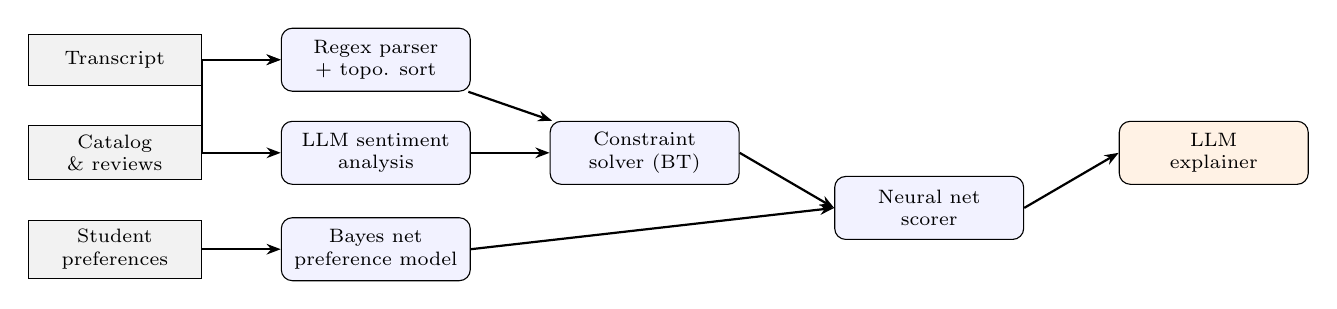
\begin{tikzpicture}[
      node distance=5mm and 6mm,
      every node/.style={font=\scriptsize},
      box/.style={
        draw, rounded corners, align=center,
        minimum width=2.4cm, minimum height=0.8cm,
        fill=blue!5
      },
      data/.style={
        draw, align=center,
        minimum width=2.2cm, minimum height=0.65cm,
        fill=gray!10
      },
      arrow/.style={-{Stealth[length=1.8mm]}, thick}
    ]
    \node[data] (transcript) {Transcript};
    \node[data, below=of transcript] (catalog) {Catalog\\\& reviews};
    \node[data, below=of catalog] (prefs) {Student\\preferences};

    \node[box, right=10mm of transcript] (parser) {Regex parser\\+ topo. sort};
    \node[box, right=10mm of catalog] (sentiment) {LLM sentiment\\analysis};
    \node[box, right=10mm of prefs] (bayes) {Bayes net\\preference model};

    \node[box, right=10mm of sentiment] (csp) {Constraint\\solver (BT)};
    \node[box, right=12mm of csp, yshift=-7mm] (nn) {Neural net\\scorer};

    \node[box, right=12mm of nn, yshift=7mm, fill=orange!10] (llm) {LLM\\explainer};

    \draw[arrow] (transcript) -- (parser);
    \draw[arrow] (catalog)    -- (sentiment);
    \draw[arrow] (catalog.east)    |- (parser.west);
    \draw[arrow] (prefs)      -- (bayes);
    \draw[arrow] (parser)     -- (csp);
    \draw[arrow] (sentiment)  -- (csp);
    \draw[arrow] (csp.east)   -- (nn.west);
    \draw[arrow] (bayes.east) -- (nn.west);
    \draw[arrow] (nn.east)    -- (llm.west);
  \end{tikzpicture}
  \caption{End-to-end pipeline. Gray nodes are data sources; blue nodes are
    deterministic / model components; the orange node is the LLM explainer
    that closes the loop with the user.}
  \label{fig:pipeline}
\end{figure*}

\subsection{Prerequisite Parsing and Topological Sort}

Each prerequisite string in the scraped catalog is tokenized by a regular
expression that recognizes course mnemonics (\code{CS\,2110}), boolean
operators (\code{and}, \code{or}, commas, parentheses), and a handful of
special phrases. The resulting AND/OR tree is normalized into disjunctive
normal form so that the solver can ask the cheap question
``does \emph{at least one} clause's literals all appear in the student's
completed-course set?''.

Course nodes are then topologically sorted on the AND-edges of the DAG,
producing a per-student \emph{eligibility frontier}: the set of courses the
student is currently allowed to take. This frontier is recomputed lazily on
each backtracking step in the solver, allowing the solver to plan multi-
semester sequences when desired.

\subsection{LLM Sentiment Analysis Over Reviews}

For each course section, we collapse all available reviews into a single
prompt and ask a local Qwen~2.5 7B model to emit a structured JSON object
with four scalars in $[0,1]$:
\begin{itemize}[leftmargin=*,topsep=1pt,itemsep=1pt]
  \item \code{difficulty} -- conceptual hardness of the material;
  \item \code{workload} -- time commitment per week;
  \item \code{enjoyability} -- overall student satisfaction;
  \item \code{instructor\_efficacy} -- teaching quality of the
    instructor.
\end{itemize}
Negative-sentiment phrasing (``brutal'', ``unfair'', ``hours of busywork'')
maps to high difficulty, high workload, and low enjoyability; positive
phrasing maps the opposite way. We chose an LLM over a classical
bag-of-words classifier because the reviews mix evaluative claims about
\emph{the instructor} with claims about \emph{the material}, and
disambiguating these requires sentence-level semantics that simple lexicon
methods miss.

\subsection{Constraint Solver}

The constraint solver is a depth-first backtracking search over assignments
of \emph{section} (not just course) to a schedule slot. Hard constraints
are encoded directly into the search:
\begin{itemize}[leftmargin=*,topsep=1pt,itemsep=1pt]
  \item \emph{No time conflicts.} Sections expose a list of meeting
    intervals; pairwise overlap is checked at insertion time, pruning entire
    subtrees early.
  \item \emph{Prerequisites satisfied.} The DNF clause produced by the
    parser is checked against the student's completed-course set and
    courses already placed earlier in the schedule.
  \item \emph{User-defined unavailable blocks.} Students can mark times as
    off-limits (\eg{} a part-time job).
  \item \emph{Credit range.} The total credit count must lie in
    $[c_{\min}, c_{\max}]$; partial assignments outside this range are
    pruned.
\end{itemize}
Within these hard constraints, the solver enumerates feasible schedules and
forwards each to the scoring stack. Currently the solver collects
schedules until a manually configured cap is reached; we discuss this
limitation in Section~\ref{sec:conclusion}.

\subsection{Bayesian Network for Preference Modeling}

The Bayes net (Figure~\ref{fig:bayesnet}) models the joint distribution
\[
  P(E \mid M, D, P, T)
\]
where $E$ is the latent ``enjoyment'' variable for a candidate course,
$M$ is the student's major, $D$ is the course's inferred difficulty (from
the sentiment stage), $P$ is the course's instructor-efficacy posterior,
and $T$ is the student's stated topical preferences. Conditional probability
tables are populated from the synthetic review dataset and from a small
set of hand-encoded priors (\eg{} students who self-report wanting an
``easier'' semester have a lower prior on enjoying high-difficulty
courses).

\begin{figure}[t]
  \centering
  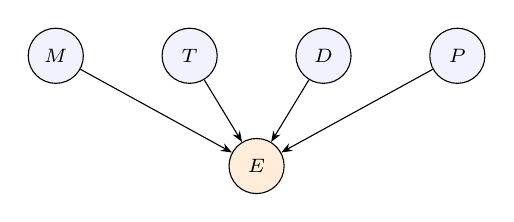
\begin{tikzpicture}[
      every node/.style={font=\scriptsize},
      var/.style={
        draw, circle, minimum size=7mm, inner sep=0pt, fill=blue!5
      },
      latent/.style={
        draw, circle, minimum size=7mm, inner sep=0pt,
        fill=orange!15
      },
      arrow/.style={-{Stealth[length=1.4mm]}}
    ]
    \node[var] (M) at (0,0) {$M$};
    \node[var] (T) at (1.7,0) {$T$};
    \node[var] (D) at (3.4,0) {$D$};
    \node[var] (P) at (5.1,0) {$P$};
    \node[latent] (E) at (2.55,-1.4) {$E$};

    \draw[arrow] (M) -- (E);
    \draw[arrow] (T) -- (E);
    \draw[arrow] (D) -- (E);
    \draw[arrow] (P) -- (E);
  \end{tikzpicture}
  \caption{Bayes net used for per-course preference scoring. Observed
    variables (blue) condition the latent enjoyment posterior $E$ (orange).}
  \label{fig:bayesnet}
\end{figure}

The Bayes net is intentionally shallow. A deeper structure would have
required substantially more data to fit reliably; the current shape gives
us a closed-form posterior per course in microseconds, which is critical
because the neural network downstream queries the Bayes net for every
section in every candidate schedule.

\subsection{Neural Network Schedule Scorer}

Where the Bayes net scores a single course in isolation, the neural
network scores an \emph{entire schedule}. Its input is a fixed-length
feature vector containing:
\begin{itemize}[leftmargin=*,topsep=1pt,itemsep=1pt]
  \item per-course Bayes-net posteriors,
  \item aggregate statistics (total credits, mean difficulty, variance of
    daily workload),
  \item indicator features for distribution requirements satisfied,
  \item alignment with the student's stated credit and difficulty range.
\end{itemize}
The network is a small two-hidden-layer MLP (64$\to$32 ReLU) with a sigmoid
output interpreted as an overall ``schedule fit'' score in $[0,1]$. Training
labels were generated by combining ground-truth feasibility with
heuristically-scored preference fit, then iteratively refined as the team
flagged outputs that ``looked wrong''.

\subsection{LLM Explainer}

Finally, we pass the top-scoring schedule (and the inputs that produced it)
to an Ollama-hosted Qwen~2.5 7B model running on UVA's Rivanna HPC cluster.
The explainer's job is \emph{not} to second-guess the schedule but to
articulate, in plain English, \emph{why} each course was chosen given the
student's preferences. As discussed in Section~\ref{sec:experiments}, we
found that the prompt structure dominates output quality; the final
production prompt is a fixed template with explicit slots for
\code{class\_fit}, \code{difficulty\_match}, and
\code{professor\_rating}, which the model fills in per course.

% ==============================================================================
\section{Experiments}
\label{sec:experiments}
% ==============================================================================

We ran two targeted experiments to harden the pipeline.

\subsection{CS vs.\ Non-CS Class Balance}

\paragraph{Observation.} On internal test profiles for CS-major students,
the unbiased scorer consistently produced schedules whose CS content was
too low -- typically 1--2 CS courses out of 4--5. Manual inspection
revealed two compounding causes: (i)~the synthetic review distribution had
slightly higher mean enjoyability for general-education subjects, and
(ii)~the Bayes net's $T$ (topic) variable did not strongly enough propagate
the major signal $M$.

\paragraph{Intervention.} We added an explicit \emph{major-affinity bonus}
to the schedule-level feature vector consumed by the neural network: a
positive contribution proportional to the fraction of credits inside the
student's declared major, and a small over-indexing penalty that activates
when the fraction of \emph{out-of-major} credits exceeds a threshold. We
deliberately implemented this as a feature rather than a post-hoc filter so
the network could still trade major fit against other signals when the
trade-off was clearly favorable (\eg{} a strongly preferred elective).

\subsection{Structured vs.\ Blind Prompting for the LLM Explainer}

\paragraph{Observation.} Our initial explainer prompt was a ``blind'' dump
of the schedule, transcript, and preferences with the bare instruction
``\emph{explain why this schedule is good}''. The model produced fluent but
generic prose -- frequently repeating the same justification across courses
and occasionally hallucinating professor names or course numbers.

\paragraph{Intervention.} We replaced the blind prompt with a structured
template that requires the model to fill in, per course, three named slots:
\code{class\_fit} (one sentence on topical alignment),
\code{difficulty\_match} (one sentence on workload/difficulty fit), and
\code{professor\_rating} (one sentence on instructor efficacy, sourced
from the sentiment posterior). The template constrains both the surface
form and the content of the explanation, making it materially harder for
the model to invent ungrounded claims.

% ==============================================================================
\section{Results}
% ==============================================================================

\paragraph{End-to-end behavior.} On a representative junior-year CS profile
with a 12--15 credit target, the full pipeline returns a 15-credit,
conflict-free schedule with a neural-net schedule score of \textbf{0.68}.
Search-to-first-feasible-schedule is sub-second on commodity hardware, and
the LLM explainer (running on Rivanna) returns a complete explanation in
roughly 4--7 seconds.

\paragraph{Effect of the major-affinity term.} Table~\ref{tab:bias}
summarizes the average composition of recommended schedules for ten
synthetic CS-major profiles, before and after introducing the
major-affinity feature. The intervention shifts the CS share from 28\,\%
to 56\,\% on average without sacrificing schedule scores -- in fact the
mean schedule score improves slightly, because the network had been
penalizing the unbalanced schedules it was producing.

\begin{table}[t]
  \centering
  \small
  \caption{Average schedule composition for 10 synthetic CS-major
    profiles, before and after adding the major-affinity feature.}
  \label{tab:bias}
  \begin{tabular}{lccc}
    \toprule
    & \textbf{CS share} & \textbf{Score} & \textbf{Conflicts} \\
    \midrule
    No bias term       & 0.28 & 0.61 & 0 \\
    With bias term     & \textbf{0.56} & \textbf{0.68} & 0 \\
    \bottomrule
  \end{tabular}
\end{table}

\paragraph{Effect of the structured explainer.}
Table~\ref{tab:explainer} shows a qualitative comparison between the blind
and structured explainer prompts on a fixed schedule. The blind prompt
produces a single paragraph with course-agnostic justifications; the
structured prompt produces a per-course breakdown that references both the
sentiment-derived professor rating and the student's declared difficulty
preference. We did not run a formal user study, but each team member rated
the structured outputs as ``substantially more useful'' on
$\geq$\,8\,/\,10 sampled schedules.

\begin{table}[t]
  \centering
  \small
  \caption{Qualitative comparison of explainer prompting styles on the
    same 15-credit schedule.}
  \label{tab:explainer}
  \begin{tabular}{p{0.46\columnwidth} p{0.46\columnwidth}}
    \toprule
    \textbf{Blind prompt} & \textbf{Structured template} \\
    \midrule
    Generic, often
    duplicated across courses; occasional hallucinated instructor names. &
    Per-course paragraph with explicit \code{class\_fit},
    \code{difficulty\_match}, and \code{professor\_rating} slots filled
    from the pipeline. \\
    \bottomrule
  \end{tabular}
\end{table}

\paragraph{Failure modes.} The system has two notable failure modes.
First, when the eligibility frontier is small (\eg{} a student with a
sparsely satisfied prerequisite tree), the constraint solver can exhaust
the feasible space quickly and the network is asked to score schedules
that are all roughly equivalent; the explainer's output then under-
differentiates between candidates. Second, the neural network was trained
on heuristically-labeled data, so its absolute calibration is approximate;
a score of 0.68 is meaningful relative to other 15-credit schedules for
the same student, but should not be compared across student profiles.

% ==============================================================================
\section{Conclusion and Future Work}
\label{sec:conclusion}
% ==============================================================================

We presented an AI Course Scheduler that converts the painful, manual
process of building a semester schedule into a one-shot, explained
recommendation. The system's central design choice -- separating hard
feasibility (constraint solver) from soft preference (Bayes net + neural
network) and using LLMs only at the boundary (review sentiment, output
explanation) -- proved durable: it kept each component simple enough to
debug independently, and it isolated the LLM's well-known reliability
issues (hallucination, inconsistent constraints) from the parts of the
pipeline that must produce correct, conflict-free output.

\paragraph{Lessons learned.} The two experiments report a recurring theme:
naive, monolithic uses of either learned models or LLMs underperform
\emph{structured} uses. The major-affinity feature is essentially a
hand-crafted prior nudging the network toward globally sensible
distributions of credits; the structured explainer prompt is a hand-crafted
schema preventing the LLM from drifting into generic prose. In both cases,
the AI components do most of the work, but a small amount of explicit
structure makes the difference between a research demo and something a
student would plausibly use.

\paragraph{Future work.} The most pressing limitation is the constraint
solver itself: it is a textbook backtracking search and does not implement
constraint propagation (AC-3, MRV, LCV) or symmetry breaking, so on densely
constrained semesters it must be terminated manually after collecting a
fixed number of schedules. A future iteration should add proper
propagation, and ideally extend the constraint vocabulary to include
\emph{geographic} factors -- the walking distance between consecutive
classroom buildings, which is a real and frequently cited source of
schedule pain at UVA. Other natural extensions include (i)~learning the
Bayes net CPTs from real student outcomes once data-sharing agreements
permit, (ii)~end-to-end multi-semester planning rather than single-semester
recommendation, and (iii)~a tighter feedback loop in which the student can
``reject'' a course and see the rest of the schedule re-optimized.

% ==============================================================================
\section*{Author Contributions}
% ==============================================================================

\noindent\textbf{Liam Baird.} Implemented the regex-based prerequisite
parser and the topological sort inside the constraint solver. Contributed
to synthetic data creation. \\[2pt]
\textbf{Hugo Barnes.} Project scaffolding; initial implementations of the
Bayes net and the neural network schedule scorer; Rivanna + LLM
integration; front-end design. \\[2pt]
\textbf{Alex Chen.} Web scraping of course catalog data; tuning of the
constraint solver; optimization of the Bayes net and neural network;
prompt engineering for LLM outputs. \\[2pt]
\textbf{Matthew Heilman.} Implemented the review sentiment analysis stage;
contributed to synthetic data creation; led slide deck, video, and written
report production.

% ==============================================================================
\section*{Sharing Statement}
% ==============================================================================

\noindent The team permits this report, the project video, and the
storyboard to be shared with future CS\,4710 students and with the public.
The associated source code remains private.

% ==============================================================================
\section*{Acknowledgments and Tooling Disclosure}
% ==============================================================================

\noindent We thank the CS\,4710 course staff for guidance throughout the
semester and the UVA Research Computing group for access to the Rivanna
HPC cluster, on which the LLM explainer is hosted. Anthropic's
\emph{Claude Code}~\cite{ClaudeCode} was used as a coding assistant during
development -- primarily for scaffolding boilerplate, drafting
documentation, and accelerating the integration between the Ollama-served
LLM and the rest of the pipeline. All algorithmic decisions, experiment
design, and final code review remained the responsibility of the authors.

% ==============================================================================
% References (manual thebibliography to avoid external .bib dependency)
% ==============================================================================

\begin{thebibliography}{9}
  \small

  \bibitem{UVAUndergradRecord}
  University of Virginia.
  \newblock \emph{Undergraduate Record: B.A.\ in Computer Science (BACS)}.
  \newblock \url{https://records.ureg.virginia.edu/preview_program.php?catoid=72&poid=11789},
  accessed Spring 2026.

  \bibitem{Schaerf1999}
  A.~Schaerf.
  \newblock A survey of automated timetabling.
  \newblock \emph{Artificial Intelligence Review}, 13(2):87--127, 1999.

  \bibitem{ParameswaranKoutrika2010}
  A.~Parameswaran, G.~Koutrika, B.~Bercovitz, and H.~Garcia-Molina.
  \newblock Recsplorer: Recommendation algorithms based on precedence mining.
  \newblock In \emph{Proc.\ ACM SIGMOD}, 2010.

  \bibitem{PolyzouKarypis2019}
  A.~Polyzou and G.~Karypis.
  \newblock Feature extraction for next-term prediction of poor student
    performance.
  \newblock \emph{IEEE Transactions on Learning Technologies},
    12(2):237--248, 2019.

  \bibitem{PangLee2008}
  B.~Pang and L.~Lee.
  \newblock Opinion mining and sentiment analysis.
  \newblock \emph{Foundations and Trends in Information Retrieval},
    2(1--2):1--135, 2008.

  \bibitem{Brown2020}
  T.~B.~Brown, B.~Mann, N.~Ryder, M.~Subbiah, et al.
  \newblock Language models are few-shot learners.
  \newblock In \emph{Advances in Neural Information Processing Systems
    (NeurIPS)}, 2020.

  \bibitem{TheCourseForum}
  TheCourseForum.
  \newblock \emph{University of Virginia course reviews}.
  \newblock \url{https://thecourseforum.com/}, accessed Spring 2026.

  \bibitem{Ollama}
  Ollama.
  \newblock \emph{Run large language models locally}.
  \newblock \url{https://ollama.com/}, accessed Spring 2026.

  \bibitem{ClaudeCode}
  Anthropic.
  \newblock \emph{Claude Code: an agentic coding tool that lives in the
    terminal}.
  \newblock \url{https://www.anthropic.com/claude-code}, accessed
    Spring 2026.

\end{thebibliography}

\end{document}
